\section{Atlassian:全球领先的软件开发协作云平台}

\textbf{Atlassian为全球领先的项目管理、内容协同SaaS厂商}。Atlassian是一家澳大利亚软件公司,提供面向企业业务流程的协同办公产品,多年位居Gartner企业敏捷管理魔力象限的领导者象限。Atlassian主要面向软件开发者,也向企业技术人员、知识工作者等群体扩展,为企业内部团队合作提供解决方案。财富500强中的大多数以及全球超过240,000家各种规模的公司都依赖Atlassian的解决方案来帮助他们的团队更好地合作并按时交付高质量的结果。
\begin{figure}[H]
    \caption{Atlassian位于魔力象限的领导者}
    \begin{center}
        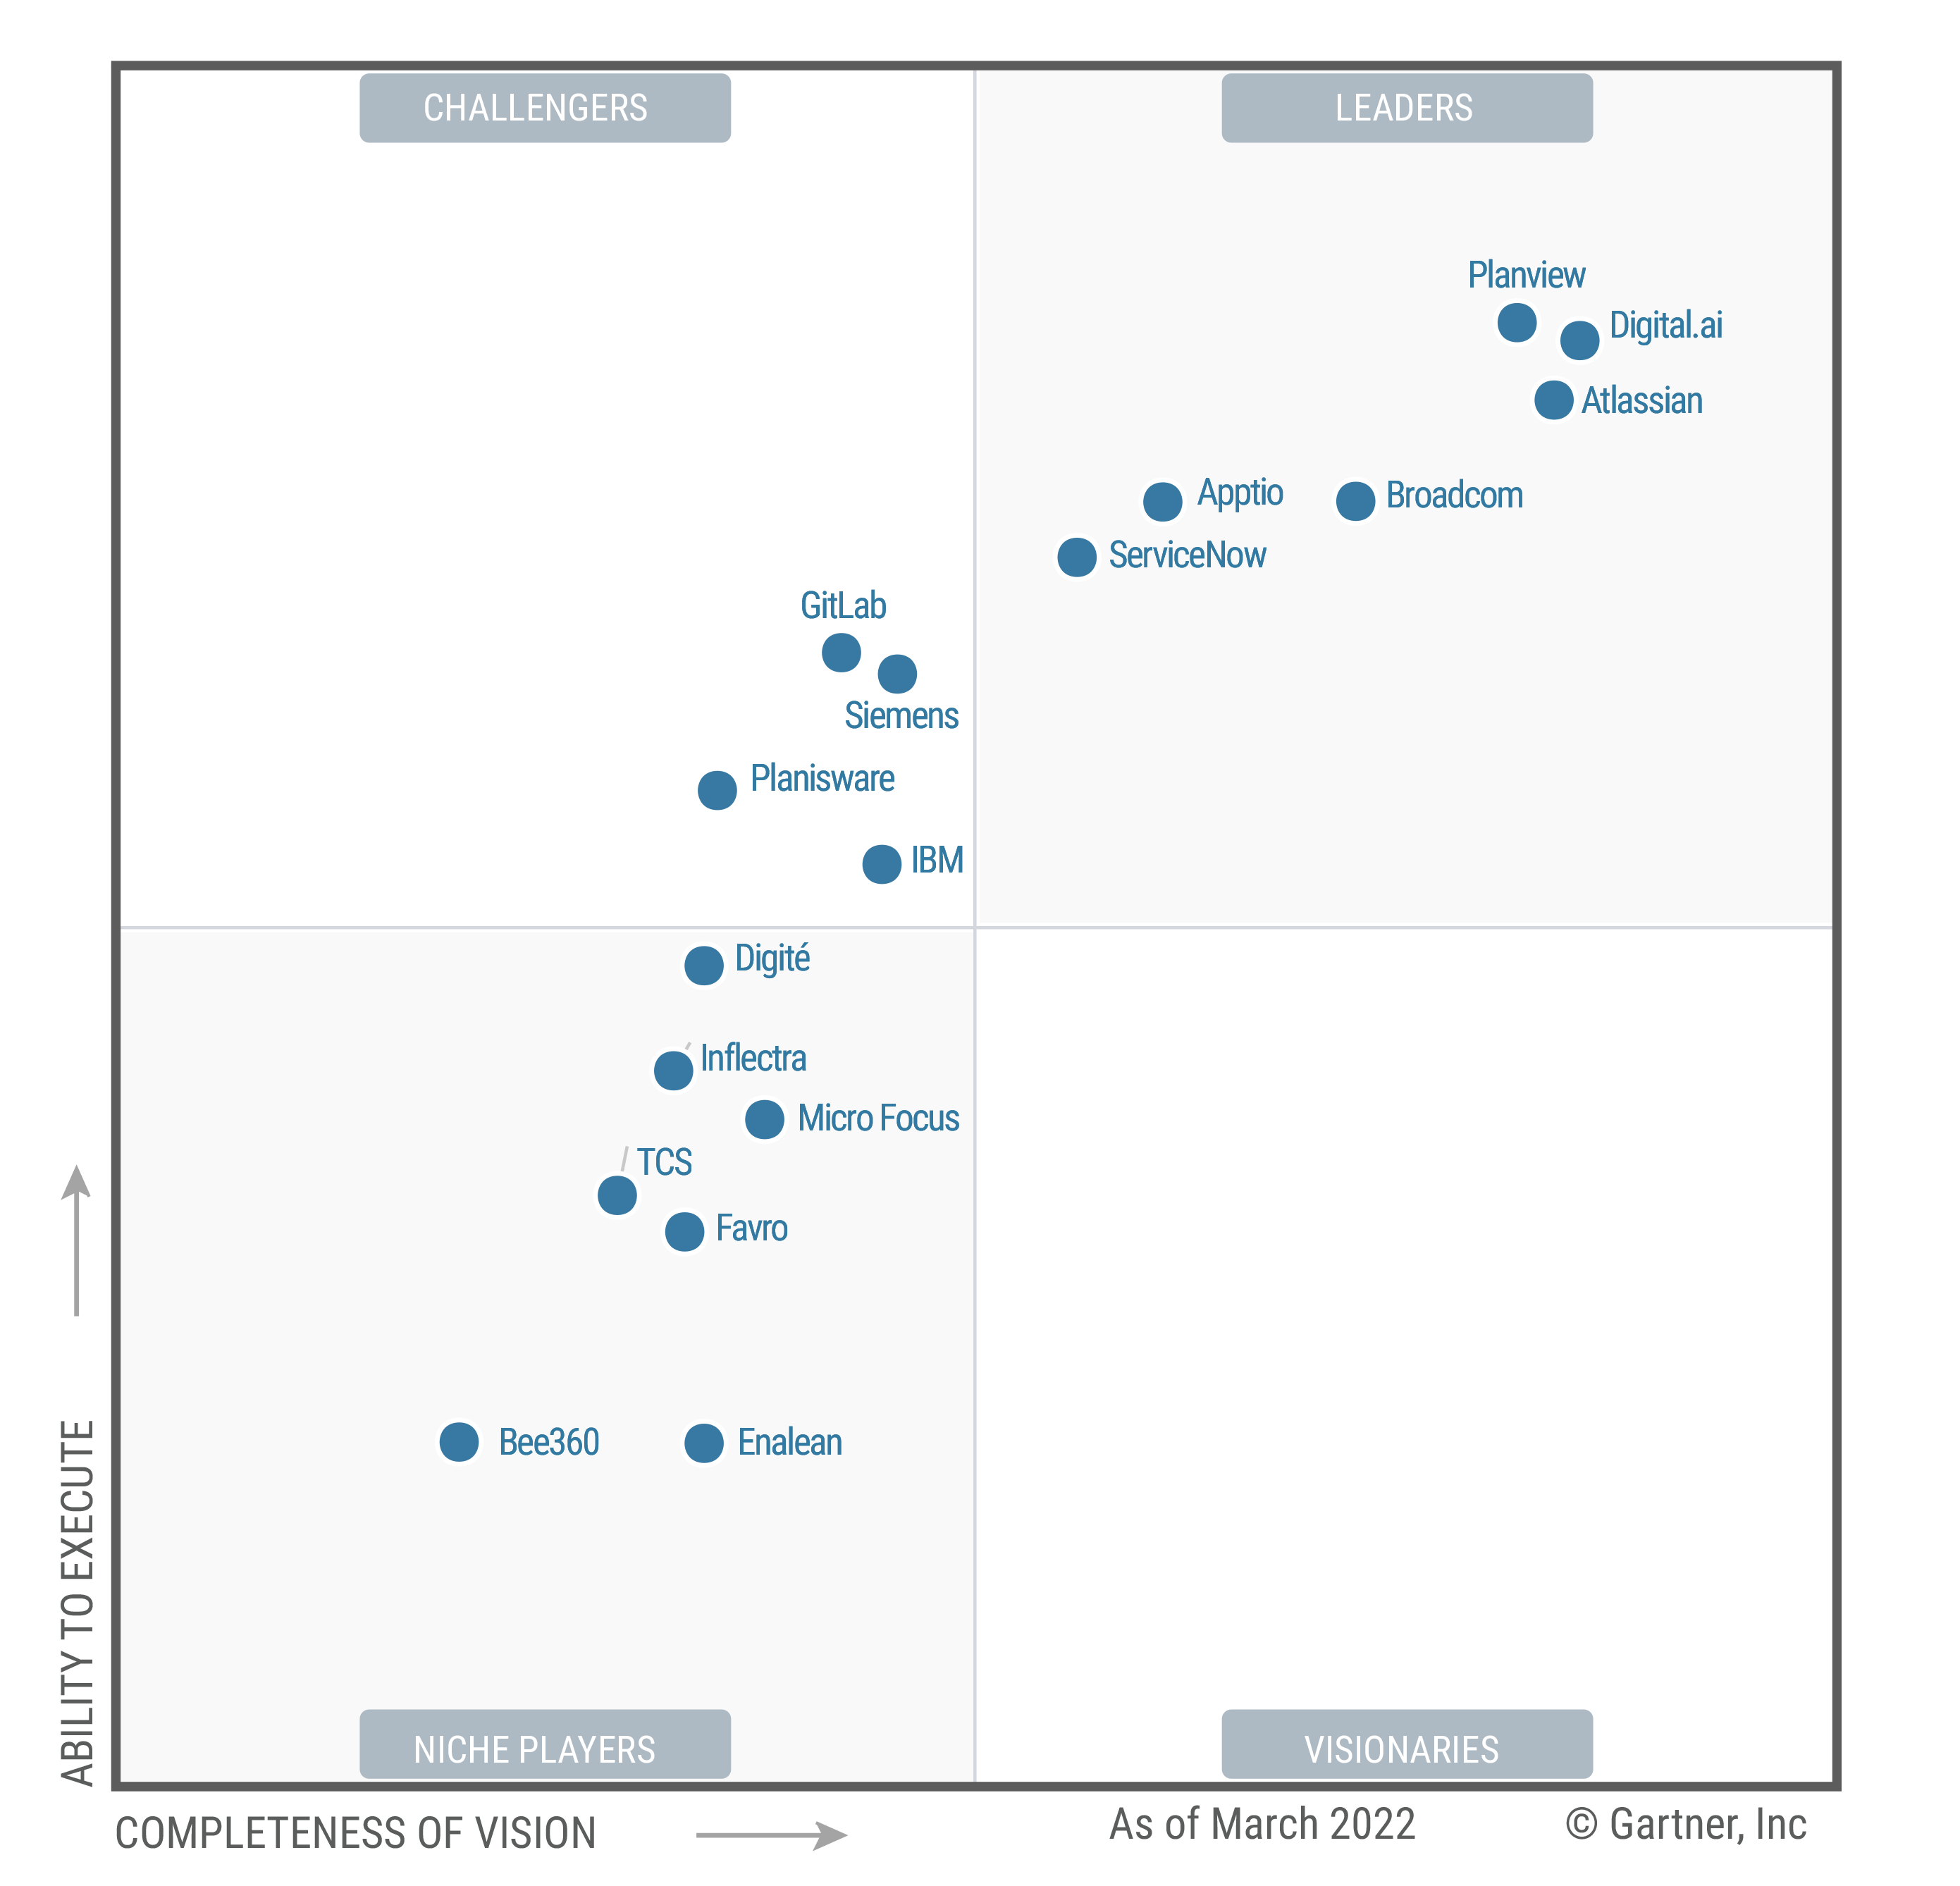
\includegraphics[width=0.5\linewidth]{img/gartner.png}
    \end{center}
    \footnotesize{资料来源:Gartner}
\end{figure}

\textbf{Atlassian 产品有非常强的用户粘性}。粘性是来自对客户业务流程的深入理解,深入到协同办公整个业务流程过程中。很好的满足了客户对业务流程管理的需要,使得团队不同成员之间的协同变得非常紧密,因而Atlassian用户保持持续增长。
\begin{figure}[H]
    \caption{Atlassian用户数}
    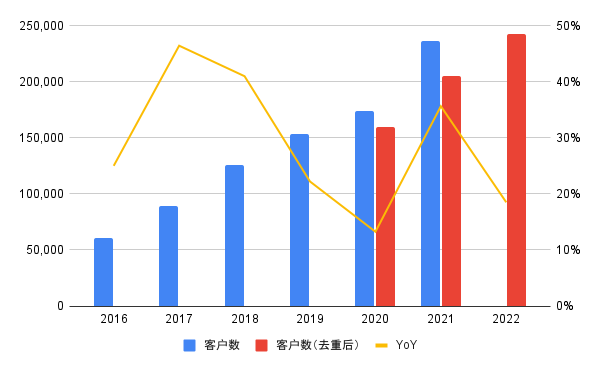
\includegraphics[width=\linewidth]{img/customers.png}
    \footnotesize{资料来源:公司公告。注:1Q22更换统计口径,对不同产品的相同用户去重}
\end{figure}

\textbf{Jira和Confluence是Atlassian的核心产品,公司专注于满足软件开发者敏捷开发与DevOps、IT服务管理和工作管理等需求}。Atlassian公司成立于2002年,在成立两年内发布了拳头产品Jira和Confluence,并在2010年将产品迭代上云,于2015年上市。伴随敏捷开发在软件开发中快速普及,依托自动化工具实现软件开发项目全流程的动态跟踪、管理成为必然趋势,Atlassian的产品受到广泛欢迎。Atlassian还通过不断并购扩大产品矩阵,如项目管理软件Trello、代码托管网站Bitbucket、Git客户端SourceTree等。这些软件都与Jira和Confluence高度集成,形成丰富的DevOps产品生态。
\begin{figure}[H]
    \caption{Atlassian公司历史}
    \begin{center}
        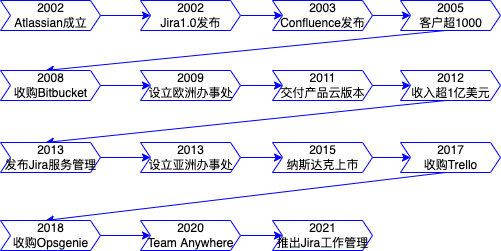
\includegraphics[width=\linewidth]{img/timeline.drawio.png}
    \end{center}
    \footnotesize{资料来源:公司公告}
\end{figure}

\textbf{Atlassian也是“云为先”的公司}。Atlassian于2010年推出了云上的Jira和Confluence版本。近年来从用户部署的方式上看,用户使用云服务贡献收入占比从40\%提升至60\%,2023财年一季度云服务的同比增速超50\%。传统的部署到自建服务器上的份额则日渐萎缩。
\begin{figure}[H]
    \caption{Atlassian按不同部署收入(百万美元)}
    \begin{center}
        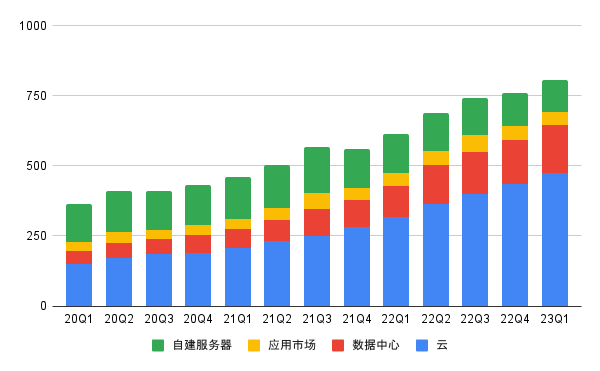
\includegraphics[width=0.8\linewidth]{img/deployment.png}
    \end{center}
    \footnotesize{资料来源:公司公告}
\end{figure}
